\setlength{\headheight}{33.24858pt}
\section*{Textbook Reference}
\begin{enumerate}[(1)]
    \item Do Carmo: Differential Geometry of Curves and Surfaces.
    \item Sebasti\'an Montiel, Antorio Ros: Curves and Surfaces.
    \item \textit{Chinese Title, add later}
\end{enumerate}
\section*{Course Introduction}
The Goal of this course is to study the ``differential geometry of curves and surfaces''.

\noindent
$\bullet$ \textbf{Geometry}: How is a geometric object curved / How to measure the curvedness of a geometric object? 
\begin{example}
     In the illustration below, (1) differs by ``topology''. In (2), they are topologically the same, while the lower curve is ``more curved'' than the upper curve.
\end{example}

\begin{center}
    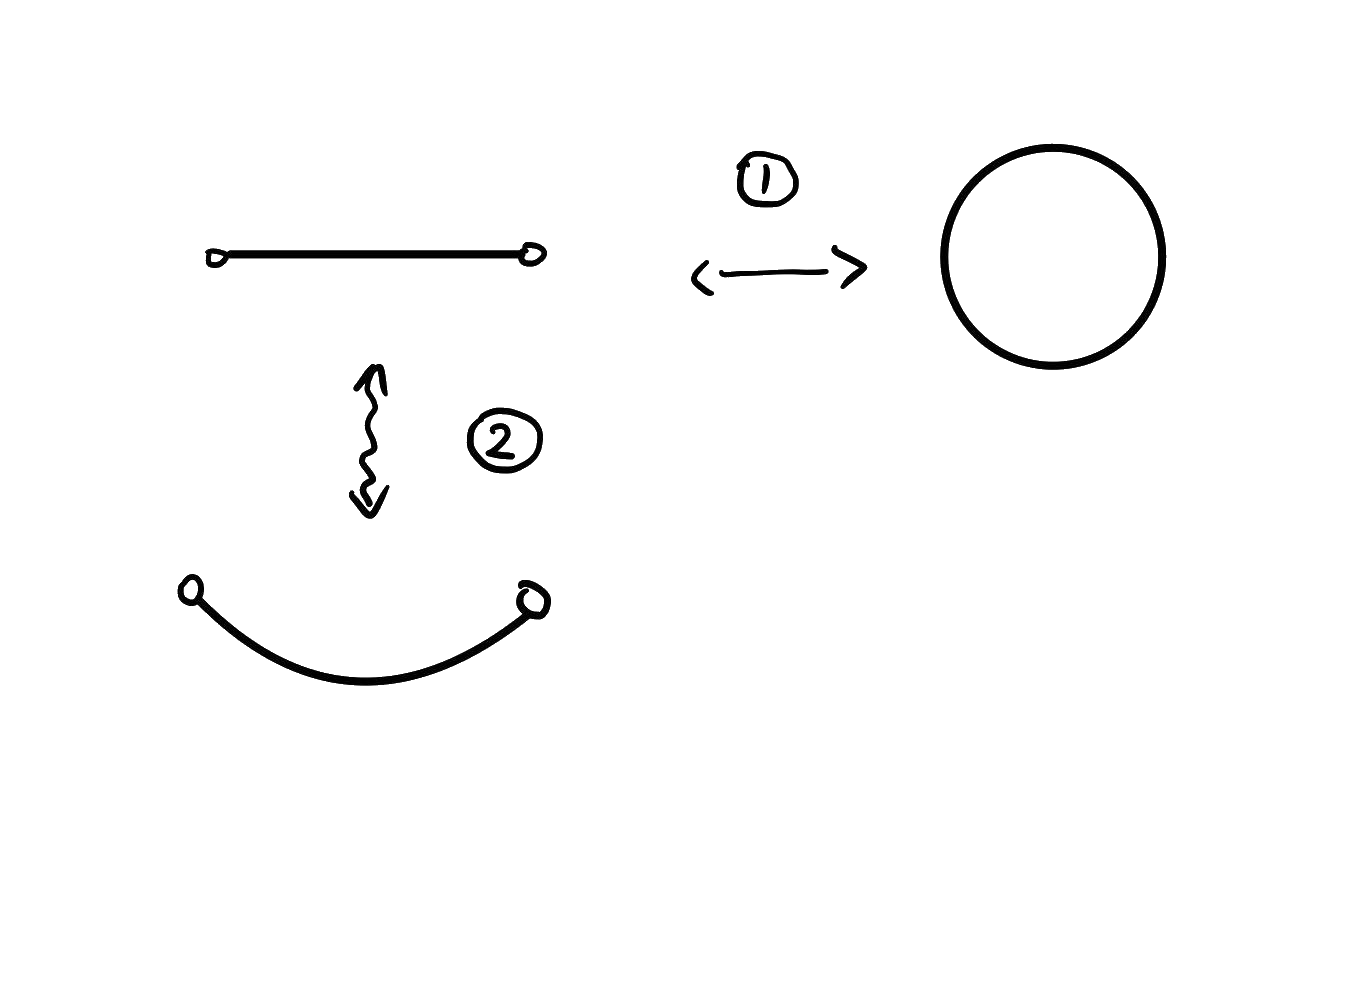
\includegraphics[scale=0.3]{picture/preface/preface_example1.png}
\end{center}

\begin{example}
    (3) differs by ``topology'', but in (4) $\mathbb{S}^2(1)$ is more curve than $\mathbb{S}^2(2)$, even topologically they are the same.(either homeomorphically or diffeomorhically).
\end{example}

\begin{center}
    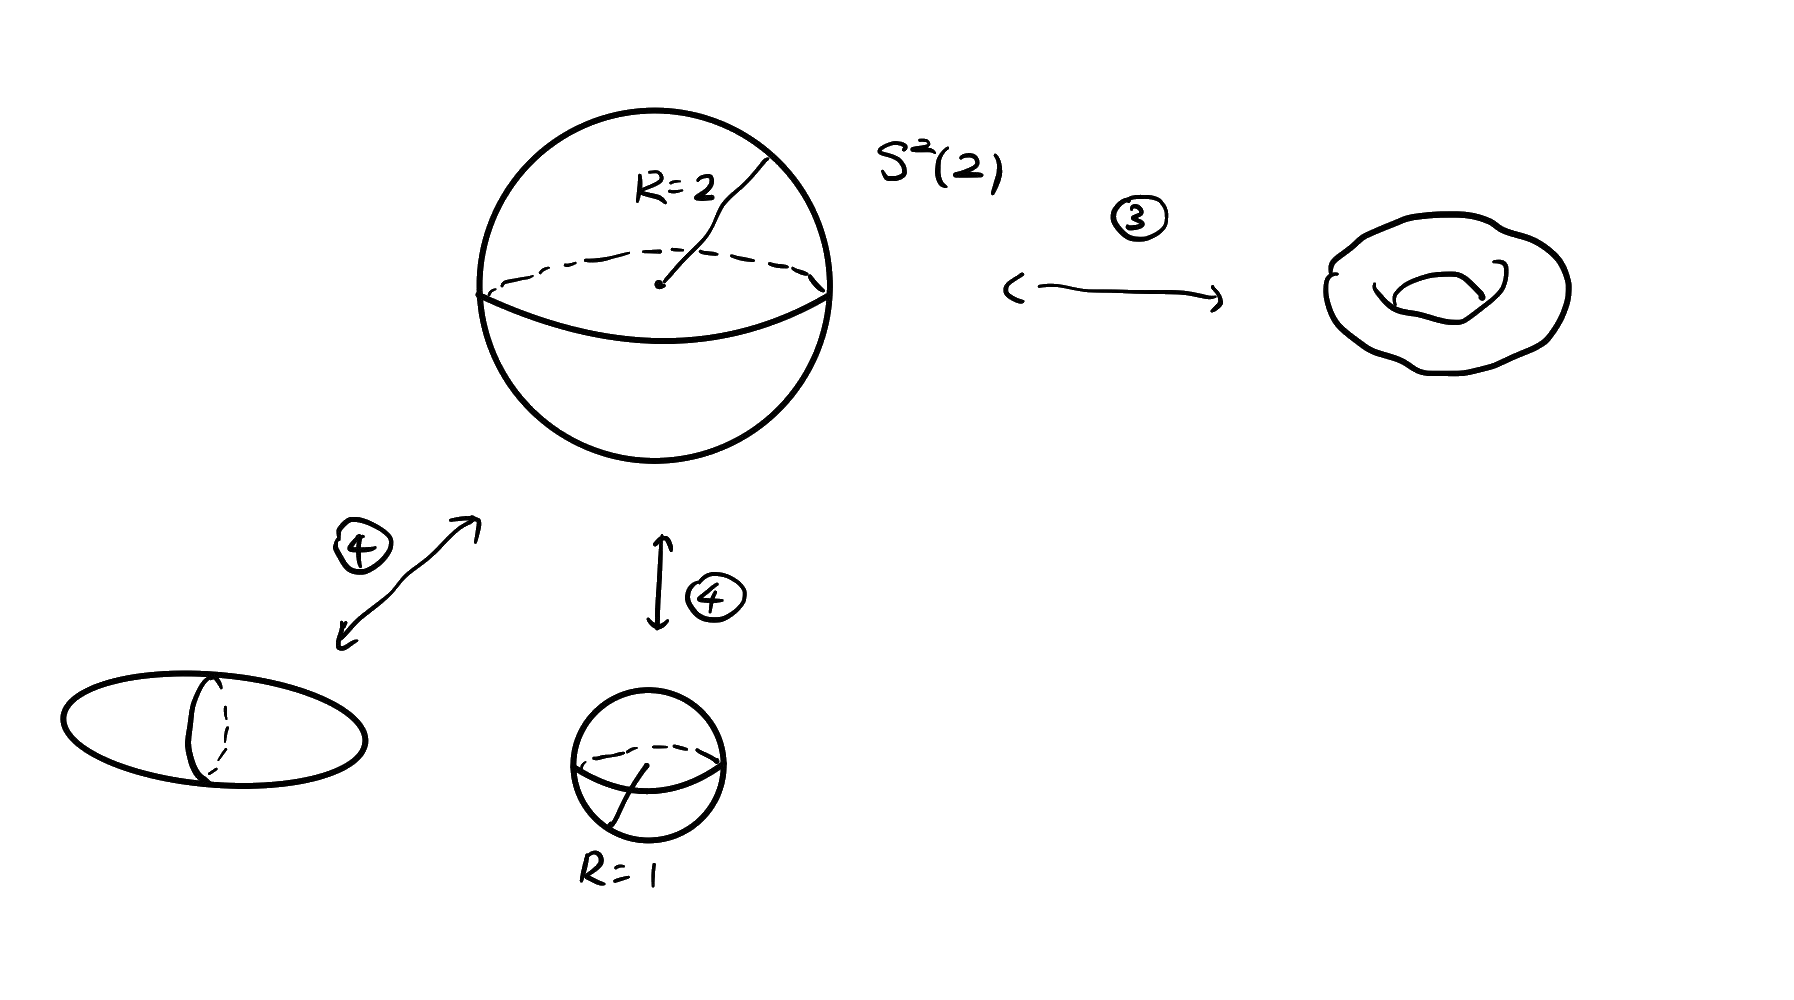
\includegraphics[scale=0.2]{picture/preface/preface_example2.png}
\end{center}

The ``Curved property'' also affects geometric quantities, like length, area, volume, angle between the curves, etc.

\textbf{Local Geometry}: How does a ``curved '' space look like in a neighborhood of a point?
 
\textbf{Global Geometry}: If we know how a ``curved space'' is look like at each point, can we observe how such space looks like globally? This is usually related to topological problems.

$\bullet$ \textbf{Differential}: In this course, by ``smoothness'' we mean the geometric objects we'll study are ``nice'' enough so we can apply ``calculus'' tools to study them.

\textbf{Main tool}: Calculus! We'll see how powerful calculus is in this course, especially, like the maximal principle, integration by parts(stoke's theorem), Taylor's expansion, implicit function theory, etc.

\begin{center}
    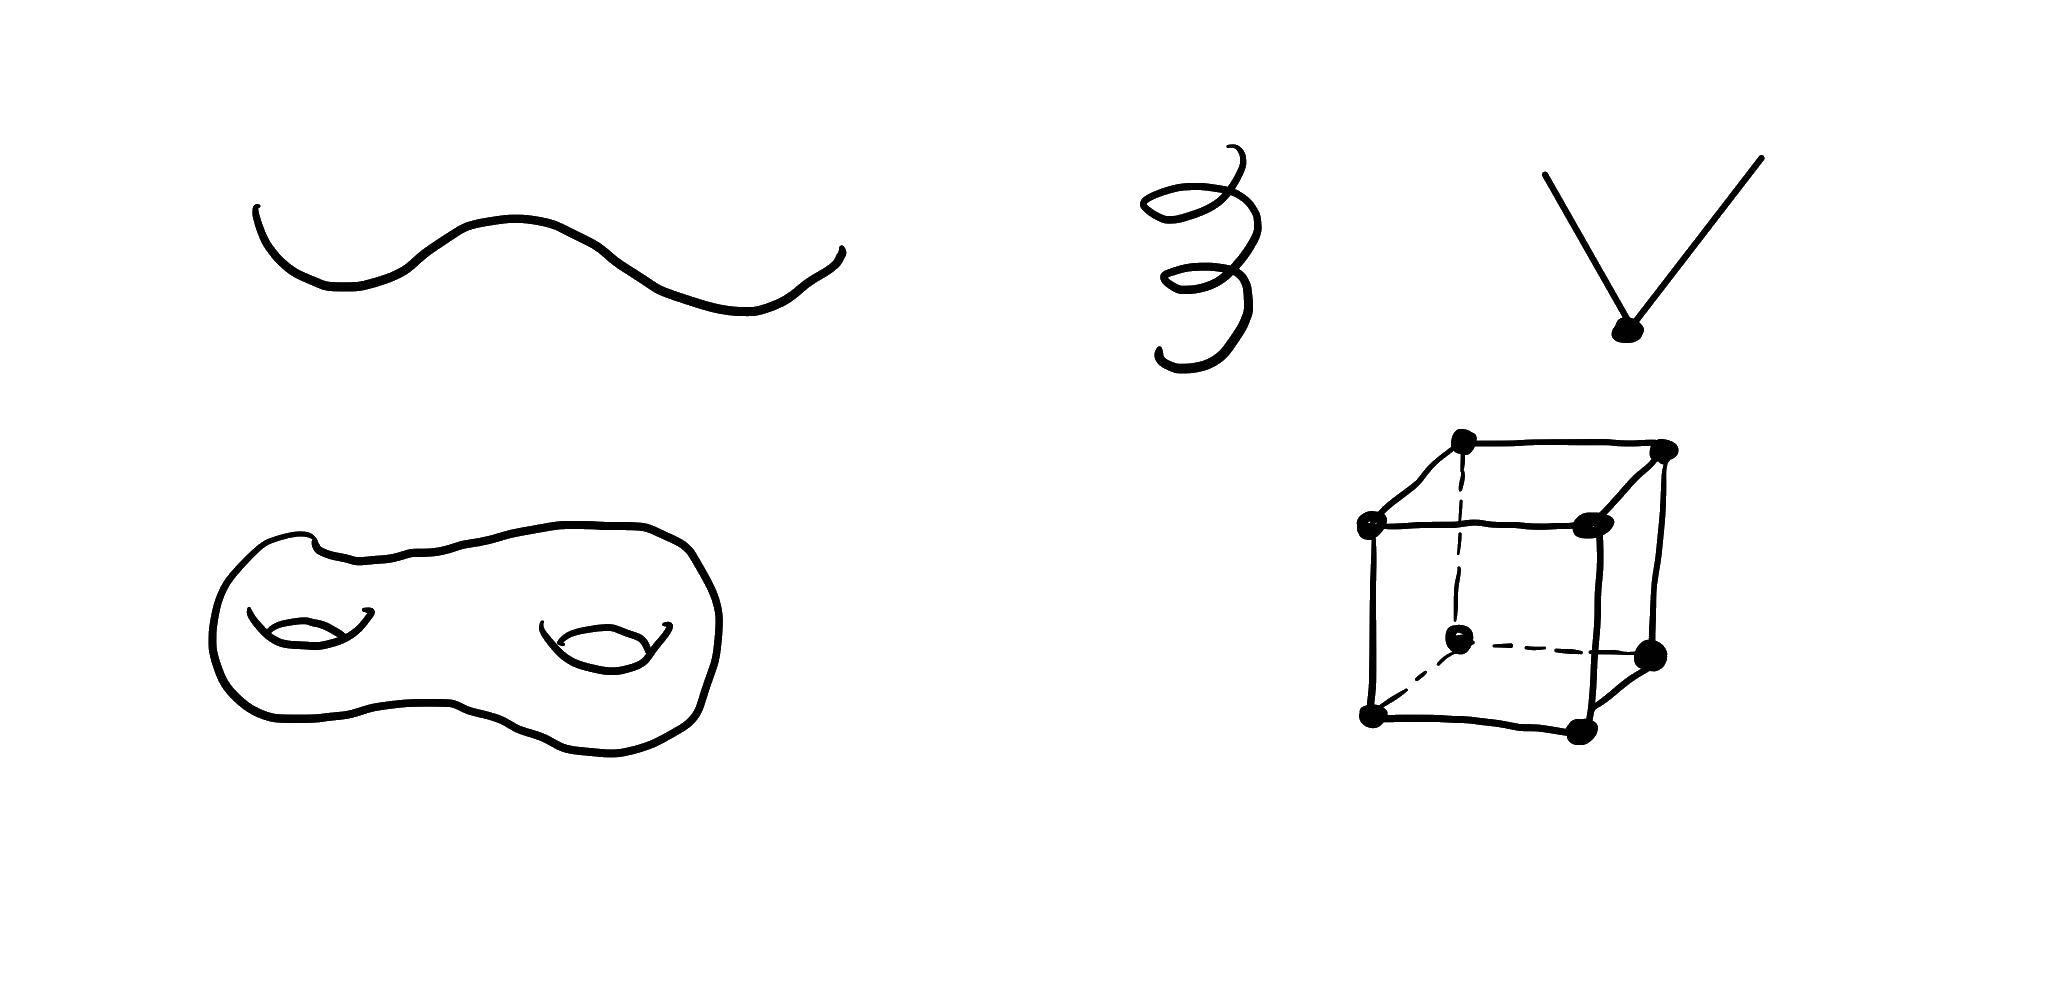
\includegraphics[scale=0.2]{picture/preface/preface_example3.png}
\end{center}

Queastion: How to tell the ``smoothness''?(Need to find good parametrization)Finding a good ``gauge''(that is ``coordinate'') to work with is also an important question in geometry.

$\bullet$Curves: 1-d geometric object.

Surfaces: 2-d geometric object.
\begin{remark}
    In this course, we only focus on curves and surfaces in $\mathbb{R}^3$.However, as a training on preparing for later geometry course, I suggest you also try to think about the ambiant space is $\mathbb{S}^3$ or $\mathbb{H}^3$.

\end{remark}
$\bullet$\textbf{Intrinsic geometry}: Study the geometric object without considering the ambient space. This begins from the Gauss's elegant theorem and was developed by Riemann.
\begin{example}
    Consider the unit sphere $\mathbb{S}^2$

    Extrinsic geometry: view it as $x^2+y^2+z^2=1$ in $\mathbb{R}^3$.

    Intrinsic geometry: $(\theta,\varphi)$ or $(\varphi,\theta)$ are ``essential'' coordinates on $\mathbb{S}^2$. \[
        \dd s^2=\dd \varphi^2+(\sin\varphi)^2 \dd\theta^2
    \]

    (Caution: $(\theta,\varphi)$ is outer normal, while $(\varphi,\theta)$ is inner normal.)
\end{example}
$\bullet$ Useful / Common techniques:
\begin{enumerate}[1)]
    \item Comparison: compare the studied geometric object with ``model space''. It's very important to study examples in geometry. As a suggestion you are expected to spend time to play with $\mathbb{S}^2$.For example: How is $\mathbb{S}^2$ curved? What's the shortest line in $\mathbb{S}^2$? How many symmetries are there on $\mathbb{S}^2$? Can you add ``extra structure'' on$\mathbb{S}^2$ to make it a complex object? Is this ``extra structure'' ``rigid''?What/s the ``moment map'' on $\mathbb{S}^2$? Does there exist a ``holomorphic'' map from $\mathbb{S}^2$ to a torus, or a surface of arbitrary genus? 
 
    If we consider an ``Energy minimizing map'' from $\mathbb{S}^2$ to $\mathbb{S}^2$, what can we say about such map?(It is  holomorphic/antiholomorphic.)
 
    After you have learned Riemann Geometry, you'll see an energy minimizing map from $\mathbb{S}^2$ to a Riemannian manifold must be an angle-preserving map(conformal map).
 
    What kinds of 2-d geometric space could be $\mathbb{S}^2$ ?(this is a global geometry problem.)(\ie\ what kinds of geometric conditions can characterize $\mathbb{S}^2$ ?)
    \item To study higher dimensional objects,it's also important to understand lower dimensional objects, and it's also important to understand lower dimensional objects contained in the studied objects.
    \item Study ``functions'' (more generally sections, including functions, vector fields, differential forms, etc.) on a given geometric object.
\end{enumerate}
\begin{example}
    On a closed surface ( $\mathbb{S}^2$,$\mathbb{T}^2$,$\Sigma_g$)(compact without boundary) there is no non-constant harmonic function.(i.e. $\Delta u=0$)(Analysis will get involved.)
\end{example}
We usually care about those functions related to geometry, such as distance functions, curvature-related functions, etc.
\begin{example}[More trivial than the last one]
    Consider $f''(x)=0$, what can you say of the solution of it when $x$ lies on a line and when $x$ lies on a circle?
\end{example}
